\newpage
\chapter{TINJAUAN PUSTAKA} \label{Bab II}

\section{Tinjauan Pustaka} \label{II.Tinjauan}
Penulis  melakukan  pencarian  referensi  terkait beberapa penelitian serupa yang pernah dilakukan sebagai dasar penelitian. Penelitian-penelitian yang menjadi referensi penulis dijabarkan pada Tabel \ref{table:2.literasi}. \par
\renewcommand{\arraystretch}{1.0} % Mengatur spasi antar baris menjadi 1
\begin{longtable}{|c|p{0.25\textwidth}|p{0.21\textwidth}|p{0.145\textwidth}|p{0.2\textwidth}|}
  \caption{Literasi Penelitian Terdahulu}\label{table:2.literasi}\\
  \hline
  \textbf{No} 
    & \textbf{Penulis [Tahun] [Judul]} 
    & \textbf{Permasalahan} 
    & \textbf{Metode} 
    & \textbf{Hasil} \\ % ← you must end the row here
  \hline
\endfirsthead
  \hline
  \textbf{No} 
    & \textbf{Penulis [Tahun] [Judul]} 
    & \textbf{Permasalahan} 
    & \textbf{Metode} 
    & \textbf{Hasil} \\ % ← and here too
  \hline
\endhead 
  \hline
\endfoot
  \hline
\endlastfoot
    1. & Yoon Kim [2014] [Convolutional Neural Networks for Sentence Classification] & Menguji efektivitas arsitektur CNN sederhana yang dilatih di atas pre-trained word vectors untuk tugas klasifikasi kalimat. & Menggunakan arsitektur CNN dengan satu lapis konvolusi dan operasi max-over-time pooling yang diaplikasikan pada word vectors. & Model CNN sederhana dengan pre-trained vectors mencapai performa yang sangat baik dan menjadi state-of-the-art di beberapa dataset. Performa ini dapat lebih ditingkatkan melalui fine-tuning.\\ 
    \hline
    2. & Bunga Aura Prameswari , Haliza Syafa Oktaviani , Titus Rangga Wicaksono, Biben Pieter Leonard, Said Achmad dan Rhio Sutoyo [2023] [Building Prediction Model for Detecting Cyberbullying using TikTok Comments ] & Membangun model prediksi untuk mendeteksi cyberbullying secara otomatis pada kolom komentar TikTok , karena fitur pencegahan yang ada saat ini masih memerlukan intervensi manual. & Menggunakan model Deep Learning dengan arsitektur BERT (Bidirectional Encoder Representations from Transformers) yang di-fine-tuning pada 1.508 komentar TikTok yang telah dikumpulkan dan dilabeli secara manual. & Model prediksi berbasis BERT berhasil mengklasifikasikan komentar cyberbullying dengan akurasi validasi mencapai 63\% , namun hasil pelatihan menunjukkan adanya indikasi overfitting. \\
    \hline
\end{longtable}




\section{Dasar Teori} \label{II.Teori}

\subsection{ Convolutional Neural Network (CNN) untuk Klasifikasi Teks} \label{II.teori1}
% Denyut yang dirasakan sebenarnya bukan darah yang dipompa langsung oleh jantung ke aorta, melainkan gelombang tekanan yang berasal dari aorta yang merambat lebih cepat dibandingkan aliran darah itu sendiri \cite{Ivanny2014Perbandingan}. \par

Convolutional Neural Network (CNN) adalah arsitektur deep learning yang terbukti efektif untuk tugas klasifikasi kalimat. Dalam konteks analisis teks, model ini bekerja dengan merepresentasikan sebuah kalimat sebagai matriks di mana setiap baris adalah vektor kata atau word embedding \cite{razi2017klasifikasi}. Lapisan konvolusi kemudian menerapkan serangkaian filter dengan ukuran kernel yang berbeda untuk mengekstrak fitur-fitur semantik dari potongan-potongan kalimat. 

Setelah itu, operasi pooling diaplikasikan untuk mengambil nilai fitur yang paling signifikan dari setiap filter, yang secara efektif menangkap sinyal terpenting dari seluruh kalimat dan mengatasi masalah panjang kalimat yang bervariasi. Fitur-fitur yang terpilih ini kemudian digabungkan dan dimasukkan ke lapisan fully connected dengan regularisasi dropout untuk menghasilkan prediksi klasifikasi melalui fungsi softmax. \par

\subsection{\textit{Pentingnya Pre-trained Word Embedding}} \label{II.teori2}
% \lipsum[1-2] % Menampilkan paragraf 1 sampai 2 dari lorem ipsum
% Gambar yang digunakan \ref{fig:3.ref_gbr}. \par
% \begin{figure}[H] % Kalau menggunakan H, posisi gambar akan tepat dibawah teks 
%     \centering
%     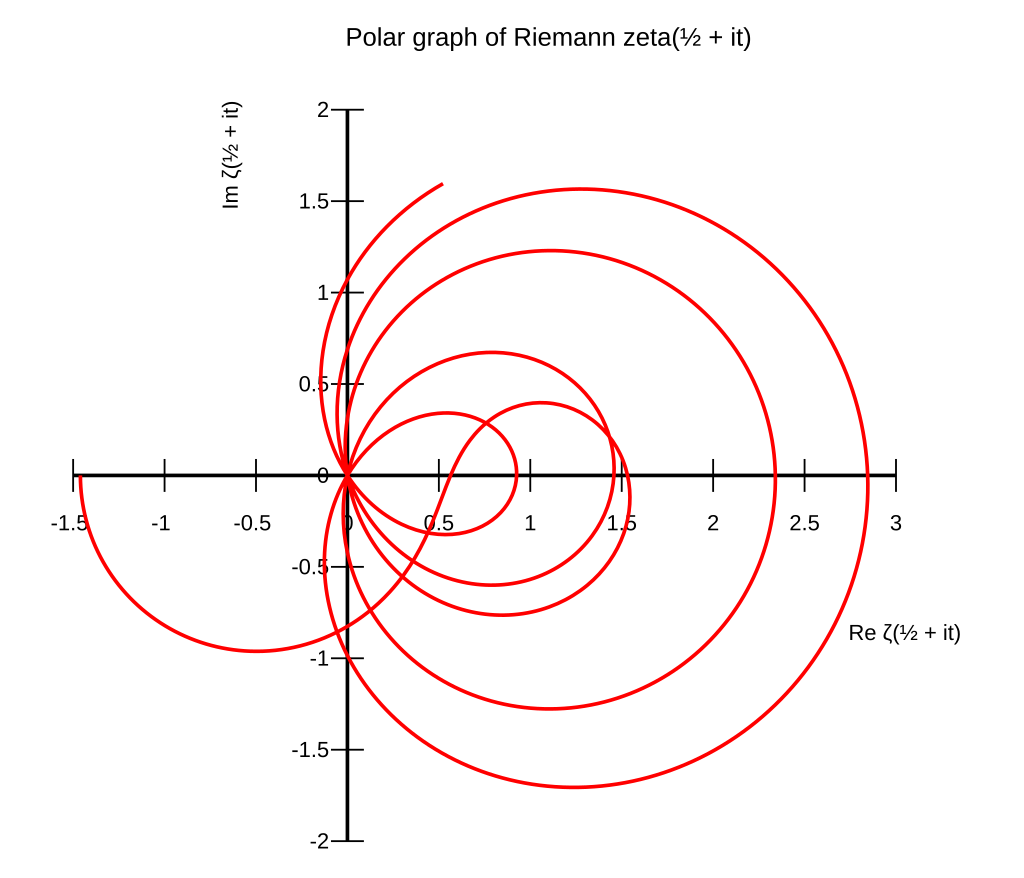
\includegraphics[width=0.6\textwidth]{figure/zeta.png}
%     \caption{Referensi Gambar}
%     \label{fig:3.ref_gbr}
%     {\footnotesize Sumber: internet}
% \end{figure}

Word embedding adalah representasi vektor dari kata-kata yang memproyeksikan makna semantik ke dalam ruang vektor berdimensi rendah, di mana kata-kata yang mirip secara makna memiliki jarak yang dekat. Penelitian oleh Yoon Kim (2014) menunjukkan bahwa menginisialisasi model CNN dengan pre-trained word embedding (vektor kata yang sudah dilatih sebelumnya pada korpus data yang sangat besar, seperti Google News) secara dramatis meningkatkan kinerja klasifikasi. 

Vektor-vektor ini berfungsi sebagai "ekstraktor fitur universal" yang kuat. Eksperimen membuktikan bahwa model dengan pre-trained vectors yang statis (tidak diubah selama pelatihan) jauh mengungguli model yang diinisialisasi secara acak. Kinerja dapat ditingkatkan lebih jauh lagi dengan melakukan fine-tuning, yaitu memperbarui nilai vektor selama proses pelatihan agar lebih spesifik dengan tugas yang dikerjakan \cite{kim2014temporal}. \par

\subsection{\textit{Analisis Sentimen}} \label{II.teori3}
% \lipsum[3-4] % Menampilkan paragraf 3 sampai 4 dari lorem ipsum
% Berikut adalah ilustrasi konsep yang digunakan seperti pada Gambar \ref{fig:3.ref_gbr2}. \par
% \begin{figure}[H] % Posisi gambar tepat dibawah teks
%   \centering
%   
\includegraphics[width=0.7\textwidth]{figure/Logo_ITERA.png}
%   \caption{Ilustrasi Konsep}
%   \label{fig:3.ref_gbr2}
%   {\footnotesize Sumber: dokumentasi penelitian}
% \end{figure}

Analisis sentimen adalah cabang dari Pemrosesan Bahasa Alami (NLP) yang bertujuan untuk mengidentifikasi, mengekstrak, dan mengklasifikasikan opini atau sentimen yang terkandung dalam sebuah teks. Tugas utamanya adalah menentukan polaritas dari teks tersebut sesuai dengan jumlah kelas yang ditentukan, apakah bernilai positif, negatif, atau netral \cite{liao2017cnn}. Pendekatan ini relevan untuk analisis komentar TikTok yang berfokus pada sentimen negatif, terutama dalam konteks cyberbullying. Dengan menggunakan CNN, model dapat belajar mengenali pola bahasa yang menunjukkan sentimen negatif, seperti kata-kata kasar, hinaan, atau komentar yang merendahkan. \par

cyberbullying di mana tujuannya adalah untuk mengklasifikasikan apakah sebuah komentar mengandung sentimen negatif yang mengarah pada perundungan.

\subsection{Cyberbullying} \label{II.mae}
% \textit{Mean Absolute Error} (MAE) \cite{Suryanto2019MAE} \cite{cort2005maermse}. Rumus perhitungan dari MAE dapat dilihat pada \ref{eq:2.mae}. \par

% \begin{equationcaptioned}[eq:2.mae]{
%     MAE = \frac{1}{n} \sum_{i=1}^{n} \left| y_i - \hat{y}_i \right|
% }{
%     Mean Absolute Error (MAE)
% }
% \end{equationcaptioned}

Cyberbullying atau perundungan siber adalah tindakan agresif dan disengaja yang dilakukan oleh individu atau kelompok menggunakan media elektronik, secara berulang-ulang terhadap seseorang yang dianggap tidak mudah untuk membela diri. Dalam konteks media sosial seperti TikTok, cyberbullying dapat bermanifestasi dalam bentuk komentar jahat, ujaran kebencian, pelecehan, atau penghinaan \cite{putri2023cyberbullying}. Analisis sentimen menggunakan model seperti Text CNN dapat diterapkan untuk mendeteksi komentar-komentar tersebut secara otomatis. Dengan melatih model pada dataset komentar yang telah dilabeli sebagai cyberbullying atau bukan, sistem dapat belajar mengenali pola bahasa yang digunakan dalam perundungan dan membantu proses moderasi konten.\par